%In de besprekeking ga ik het volgende aanhalen:
%-Aanhalen van de verschillende technologieen
%-Het onderbouwen waarom ik zo te werk ben gegaan -> hier worden de bronnen gebruikt
\chapter{Bespreking}
De structuur die in Hoofdstuk~\ref{hfdst:situering} werd opgebouwd
In de loop van dit hoofdstuk zullen de verschillende technologieën besproken worden die in aanmerking komen.
Naar het einde van het hoofdstuk toe, zal een keuze gemaakt worden en zal voor iedere component de meest geschikte technologie gekozen worden.

\section{Packager}
De eerste component die besproken wordt is de packager.
Zoals reeds besproken, moet tijdens het ontwerpen van deze component rekening gehouden worden met enkele eigenschappen.
Alvorens bepaald wordt welke technologie geschikt is, moet onderzocht worden wat ingepakt moet worden en op welke manier.
Om een correct werkende applicatie te hebben, heeft het Python raamwerk verschillende drivers en bibliotheken nodig.
\citet{Obreshkov2008244} bespreekt hoe het ATLAS project te werk gaat bij het inpakken van alle nodige software.
Het ATLAS project gebruikt CMT als configuratie manager.
Met behulp van een configuratie bestand weten verscheidene tools hoe ze een pakket moeten afhandelen \citep{Obreshkov2008244}.
Een gelijkaardige structuur is wenselijk voor het probleem.
Net zoals \citet{Obreshkov2008244} zou er voor ieder bibliotheek en driver een pakket voorzien worden.
Hierdoor wordt de herbruikbaarheid bevordert en kan voor ieder pakket apart behandelt worden.
%%% SAUCE gebruiken om statement te ondersteunen
\citet{packAtlas} spreekt ook over CMT als informatiebron voor het ophalen van meta-data.
Aan de hand van deze data kan een Pacman pakket geproduceerd worden.
Met behulp van een "Pacman file" is geweten hoe de ingepakte software behandelt moet worden.

In voorbereiding op het academiejaar, was het mogelijk om een stage te lopen bij het bedrijf.
Het doel van deze stage was het voorbereiden van de thesis.
Tijdens deze voorbereiding, werd er vooral gezocht naar een goede technologie die gebruikt kon worden voor de packager.
In wat volgt, gaat er een opsomming volgen van de onderzochte technologieën samen met hun voor- en nadelen.

%%% LAYOUT neem ik hier subparagraph of subsection
%%% SAUCE op welke manier bron naar wix main page zetten
\subsection{WiX Toolset}
Windows installer XML Toolset is een set van build tools waarmee Windows Installer packages gemaakt kunnen worden.
Bron code wordt gecompileerd en vervolgens gelinkt om een executable te maken.
De toolset zal .msi installatie pakketten, .msm merge modules en .msp patches combineren \citep{wixToolset}.


\subsection{NSIS}


\subsection{Chocolatey}


\subsection{Qt Installer Framework}


\section{Database}
Het aantal pakketten die gebruikt gaan worden, gaan alleen toenemen.
Naast deze groei zullen ook het aantal gebruikers toenemen.
Daarom werd er geopteerd om een databank te ontwerpen.
In overleg met het bedrijf werd ervoor gekozen om MySQL te gebruiken als managementsysteem.
Het ontwerp van de databank is terug te vinden in Figuur~\vref{fig:databank}.

\begin{figure}[h!]
\centering
\makebox[0pt]{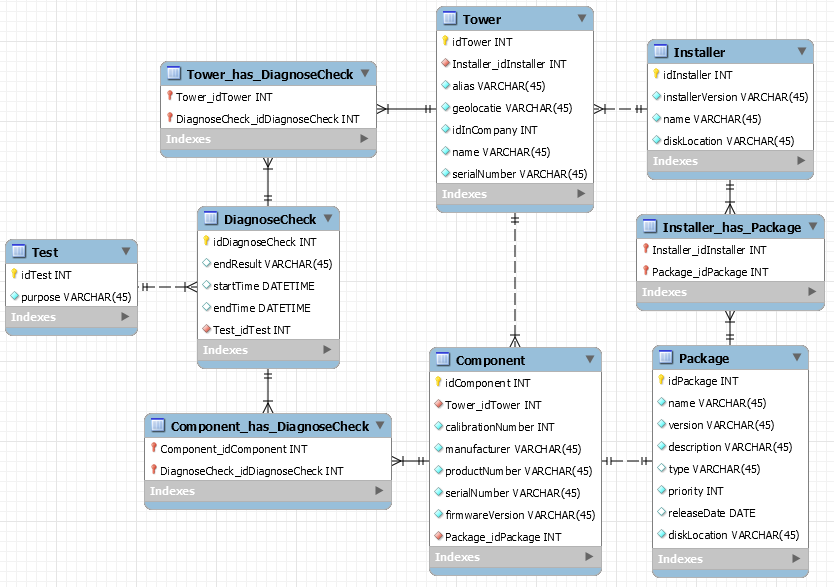
\includegraphics[scale=0.5]{afbeelding/databankOntwerp.png}}
\caption{Ontwerp van de databank}
\label{fig:databank}
\end{figure}

%bespreken van technologieen
%manier van opdeling bespreken



%\begin{figure}[!h]
%\centering
%  % We need layers to draw the block diagram
\pgfdeclarelayer{background}
\pgfdeclarelayer{foreground}
\pgfsetlayers{background,main,foreground}

% Define a few styles and constants
\tikzstyle{sensor}=[draw, fill=blue!20, text width=5em, 
    text centered, minimum height=2.5em]
\tikzstyle{ann} = [above, text width=5em]
\tikzstyle{naveqs} = [sensor, text width=6em, fill=red!20, 
    minimum height=12em, rounded corners]
\tikzstyle{naveqq} = [sensor, text width=6em, fill=red!20, 
    minimum height=2.5em, rounded corners]
\def\blockdist{2.3}
\def\edgedist{2.5}

\begin{tikzpicture}
    \node (packagerServer) [naveqs] {Packager Interface};
    % Note the use of \path instead of \node at ... below. 
    \path (packagerServer.140)+(-\blockdist,0) node (gyros) [sensor] {Rapport};
    \path (packagerServer.-150)+(-\blockdist,0) node (collect) [sensor] {Data Collector};
    
    % Unfortunately we cant use the convenient \path (fromnode) -- (tonode) 
    % syntax here. This is because TikZ draws the path from the node centers
    % and clip the path at the node boundaries. We want horizontal lines, but
    % the sensor and naveq blocks aren't aligned horizontally. Instead we use
    % the line intersection syntax |- to calculate the correct coordinate
    % We could simply have written (gyros) .. (naveq.140). However, it's
    % best to avoid hard coding coordinates
    \path [draw, ->] (collect) -- node [left] {info} 
        (collect.north |- gyros.south);
    \path [draw, <-] (collect) -- node [below] {info} 
        (packagerServer.west |- collect);    
    \node (IMU) [above of=gyros] {Status};
    \path (packagerServer.south west)+(-0.6,-0.4) node (INS) {Deployment Server};
    
    % Now it's time to draw the colored IMU and INS rectangles.
    % To draw them behind the blocks we use pgf layers. This way we  
    % can use the above block coordinates to place the backgrounds   
    \begin{pgfonlayer}{background}
        % Compute a few helper coordinates
        \path (gyros.west |- packagerServer.north)+(-0.5,0.3) node (a) {};
        \path (INS.south -| packagerServer.east)+(+0.3,-0.2) node (b) {};
        \path[fill=yellow!20,rounded corners, draw=black!50, dashed]
            (a) rectangle (b);
        \path (collect.south east)+(0.3,-0.3) node (a) {};
        \path (IMU.north -| collect.west)+(-0.3,0) node (b) {};
        \path[fill=blue!10,rounded corners, draw=black!50, dashed]
            (a) rectangle (b);
    \end{pgfonlayer}
    
    
    
	\node[below = 2cm of packagerServer] (receiver) [naveqq] {Package Receiver};
    % Note the use of \path instead of \node at ... below. 
    \path (receiver.180)+(-\blockdist,0) node (gyros) [naveqq] {Status};
    \path (receiver.270)+(0,-1.5) node (accel) [naveqq] {Unpacker};
    \path (accel.180)+(-\blockdist,0) node (installer) [naveqq] {Installer};
    % Unfortunately we cant use the convenient \path (fromnode) -- (tonode) 
    % syntax here. This is because TikZ draws the path from the node centers
    % and clip the path at the node boundaries. We want horizontal lines, but
    % the sensor and naveq blocks aren't aligned horizontally. Instead we use
    % the line intersection syntax |- to calculate the correct coordinate
    \path [draw, ->] (gyros) -- node [left] {data} 
        (gyros |- collect.south) ;
    \path [draw, ->] (receiver) -- node [right] {New package} 
        (receiver |- accel.north) ;
	\path [draw, ->] (accel) -- node [above] {} 
        (installer.east |- accel) ;
	\path [draw, ->] (installer) -- node [right] {OK} 
        (installer |- gyros.south) ;
    \path [draw, ->] (packagerServer) -- node [above] {} 
        (packagerServer.south |- receiver.north);        
    % We could simply have written (gyros) .. (naveq.140). However, it's
    % best to avoid hard coding coordinates
    \path (accel.south west)+(-0.6,-0.4) node (INS) {Deployment Environment};


    % Now it's time to draw the colored IMU and INS rectangles.
    % To draw them behind the blocks we use pgf layers. This way we  
    % can use the above block coordinates to place the backgrounds   
    \begin{pgfonlayer}{background}
        % Compute a few helper coordinates
        \path (gyros.west |- receiver.north)+(-0.5,0.3) node (a) {};
        \path (INS.south -| receiver.east)+(+0.3,-0.2) node (b) {};
        \path[fill=yellow!20,rounded corners, draw=black!50, dashed]
            (a) rectangle (b);
    \end{pgfonlayer}
    
    
	\node[right= 4cm of packagerServer.north, anchor=north](mapper) [naveqq] {Mapper};
    % Note the use of \path instead of \node at ... below. 
    \path (mapper.-90)+(0,-1.5) node (interface) [naveqq] {Packager Interface};
    \path (mapper)+(3,0) node (accel) [naveqq] {Package Producer};
    
    % Unfortunately we cant use the convenient \path (fromnode) -- (tonode) 
    % syntax here. This is because TikZ draws the path from the node centers
    % and clip the path at the node boundaries. We want horizontal lines, but
    % the sensor and naveq blocks aren't aligned horizontally. Instead we use
    % the line intersection syntax |- to calculate the correct coordinate
%    \path [draw, ->] (gyros) -- node [above] {$\vc{\omega}_{ib}^b$} 
%        (test.west |- gyros) ;
%    % We could simply have written (gyros) .. (naveq.140). However, it's
%    % best to avoid hard coding coordinates
    \path [draw, ->] (mapper) -- node [above] {} 
        (accel.west |- mapper);
    \path [draw, ->] (accel.south) -- (interface.east);
    \path [draw, ->] (interface) -- node [above] {} 
        (packagerServer.east |- interface);
	\path (mapper.90)+(0,1.5) node (db) {Database};
    \path [draw, -] (db) -- node [above] {} 
        (db.south |- mapper.north);
    \path (interface.south east)+(0.3,-0.4) node (INS) {Packager};


    % Now it's time to draw the colored IMU and INS rectangles.
    % To draw them behind the blocks we use pgf layers. This way we  
    % can use the above block coordinates to place the backgrounds   
    \begin{pgfonlayer}{background}
        % Compute a few helper coordinates
        \path (interface.west |- mapper.north)+(-0.5,0.3) node (a) {};
        \path (INS.south -| accel.east)+(+0.3,-0.2) node (b) {};
        \path[fill=yellow!20,rounded corners, draw=black!50, dashed]
            (a) rectangle (b);
    \end{pgfonlayer}
\end{tikzpicture}
%  \caption{Blok diagram met alle componenten}
%  \label{fig:overzichtBlok}
%\end{figure}

%
%BlokSchema met de algemene structuur van de packager
%

%In het vorig hoofdstuk hebben we naar deze tekst verwezen\label{verwijzing}.